% =====================================================================
%  FIGURAS TIKZ PARA O TCC - GraphRAG Eventos Climáticos
% =====================================================================
%
%  Este arquivo contém:
%  (A) Trechos para adicionar ao PREÂMBULO do seu .tex principal
%  (B) Substituições para cada uma das três figuras
%
%  Você pode usar de duas formas:
%  1) Compilar os arquivos PDF separados (figura1_esquema_grafo.pdf etc)
%     e incluir com \includegraphics — basta substituir o \fbox{\parbox{...}}
%     por 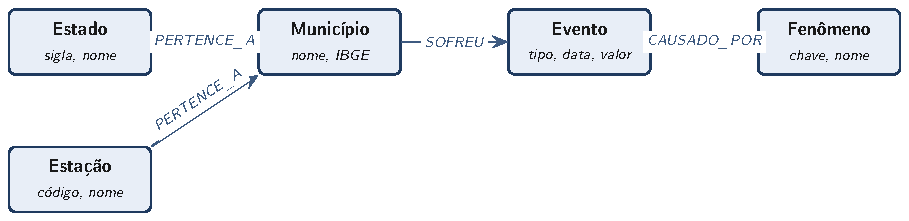
\includegraphics[width=\columnwidth]{figura1_esquema_grafo.pdf}
%
%  2) Colar os snippets TikZ diretamente no seu paper (recomendado para
%     consistência tipográfica — o TikZ usa as fontes do documento).
%
% =====================================================================

% =====================================================================
%  (A) ADICIONE AO PREÂMBULO (depois dos pacotes já existentes)
% =====================================================================

\usepackage{tikz}
\usetikzlibrary{positioning, shapes.geometric, arrows.meta, calc}

% Paleta sóbria, imprime bem em P&B
\definecolor{nodeFill}{HTML}{E8EEF7}
\definecolor{nodeStroke}{HTML}{1F3A5F}
\definecolor{accent}{HTML}{3D5A80}
\definecolor{soft}{HTML}{F4F1EA}
\definecolor{softStroke}{HTML}{8B7355}
\definecolor{decision}{HTML}{FFF4E0}
\definecolor{decisionStroke}{HTML}{B8860B}
\definecolor{textDark}{HTML}{1A1A1A}


% =====================================================================
%  (B1) SUBSTITUA \fbox{\parbox{...}} DA FIGURA "esquema_grafo"
%       (na Seção Metodologia / Grafo de Conhecimento)
% =====================================================================

\begin{figure}[htbp]
\centerline{
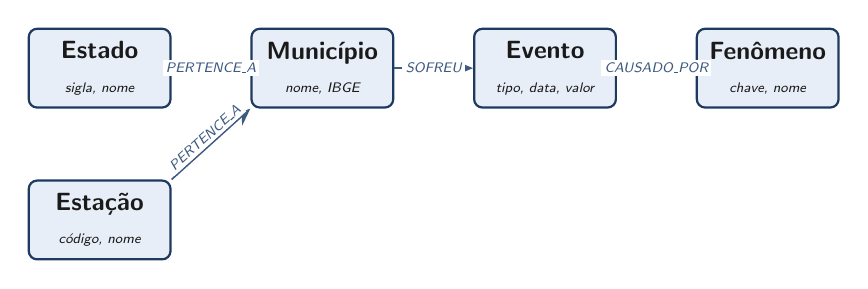
\begin{tikzpicture}[
  font=\sffamily\small,
  every node/.style={text=textDark},
  entity/.style={
    rectangle, rounded corners=3pt,
    draw=nodeStroke, line width=0.8pt,
    fill=nodeFill,
    minimum width=18mm, minimum height=10mm,
    align=center, inner sep=2pt
  },
  rel/.style={
    -{Stealth[length=2.2mm, width=1.8mm]},
    draw=accent, line width=0.6pt
  },
  rellabel/.style={
    font=\sffamily\tiny\itshape,
    text=accent, fill=white, inner sep=1.2pt
  }
]
  \node[entity] (estado) {\textbf{Estado}\\[1pt]\tiny\itshape sigla, nome};
  \node[entity, right=10mm of estado]  (municipio) {\textbf{Município}\\[1pt]\tiny\itshape nome, IBGE};
  \node[entity, right=10mm of municipio] (evento)  {\textbf{Evento}\\[1pt]\tiny\itshape tipo, data, valor};
  \node[entity, right=10mm of evento]    (fenomeno) {\textbf{Fenômeno}\\[1pt]\tiny\itshape chave, nome};
  \node[entity, below=9mm of estado] (estacao) {\textbf{Estação}\\[1pt]\tiny\itshape código, nome};

  \draw[rel] (municipio) -- (estado)
    node[rellabel, midway] {PERTENCE\_A};
  \draw[rel] (municipio) -- (evento)
    node[rellabel, midway] {SOFREU};
  \draw[rel] (evento) -- (fenomeno)
    node[rellabel, midway] {CAUSADO\_POR};
  \draw[rel] (estacao.north east) -- (municipio.south west)
    node[rellabel, midway, sloped, above] {PERTENCE\_A};
\end{tikzpicture}
}
\caption{Esquema do grafo de conhecimento climático no Neo4j.}
\label{fig:esquema_grafo}
\end{figure}


% =====================================================================
%  (B2) SUBSTITUA \fbox{\parbox{...}} DA FIGURA "pipeline"
%       (na Seção Metodologia / Pipeline GraphRAG)
% =====================================================================

\begin{figure}[htbp]
\centerline{
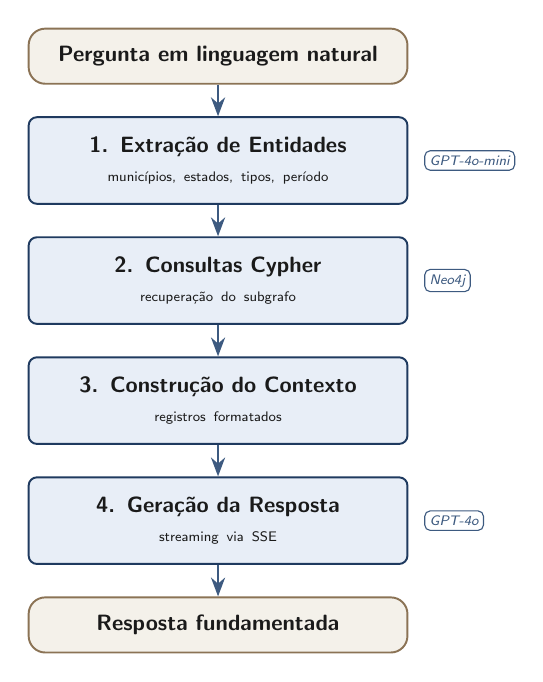
\begin{tikzpicture}[
  font=\sffamily\footnotesize,
  every node/.style={text=textDark},
  io/.style={
    rectangle, rounded corners=6pt,
    draw=softStroke, line width=0.7pt, fill=soft,
    text width=46mm, minimum height=7mm,
    align=center, inner sep=3pt
  },
  stepbox/.style={
    rectangle, rounded corners=3pt,
    draw=nodeStroke, line width=0.7pt, fill=nodeFill,
    text width=46mm, minimum height=11mm,
    align=center, inner sep=3pt
  },
  techbadge/.style={
    rectangle, rounded corners=2pt,
    draw=accent, line width=0.4pt, fill=white,
    font=\sffamily\tiny\itshape,
    text=accent, inner sep=1.8pt
  },
  flow/.style={
    -{Stealth[length=2.4mm, width=1.8mm]},
    draw=accent, line width=0.7pt
  }
]
  \node[io] (input) {\textbf{Pergunta em linguagem natural}};

  \node[stepbox, below=4mm of input] (extract)
    {\textbf{1. Extração de Entidades}\\[1pt]
     \tiny municípios, estados, tipos, período};
  \node[techbadge, right=2mm of extract] {GPT-4o-mini};

  \node[stepbox, below=4mm of extract] (cypher)
    {\textbf{2. Consultas Cypher}\\[1pt]
     \tiny recuperação do subgrafo};
  \node[techbadge, right=2mm of cypher] {Neo4j};

  \node[stepbox, below=4mm of cypher] (context)
    {\textbf{3. Construção do Contexto}\\[1pt]
     \tiny registros formatados};

  \node[stepbox, below=4mm of context] (gen)
    {\textbf{4. Geração da Resposta}\\[1pt]
     \tiny streaming via SSE};
  \node[techbadge, right=2mm of gen] {GPT-4o};

  \node[io, below=4mm of gen] (output) {\textbf{Resposta fundamentada}};

  \draw[flow] (input)   -- (extract);
  \draw[flow] (extract) -- (cypher);
  \draw[flow] (cypher)  -- (context);
  \draw[flow] (context) -- (gen);
  \draw[flow] (gen)     -- (output);
\end{tikzpicture}
}
\caption{Pipeline GraphRAG: extração de entidades, recuperação Cypher,
construção de contexto e geração de resposta.}
\label{fig:pipeline}
\end{figure}


% =====================================================================
%  (B3) SUBSTITUA \fbox{\parbox{...}} DA FIGURA "roteamento"
%       (na Seção Metodologia / Recuperação do Subgrafo)
% =====================================================================

\begin{figure}[htbp]
\centerline{
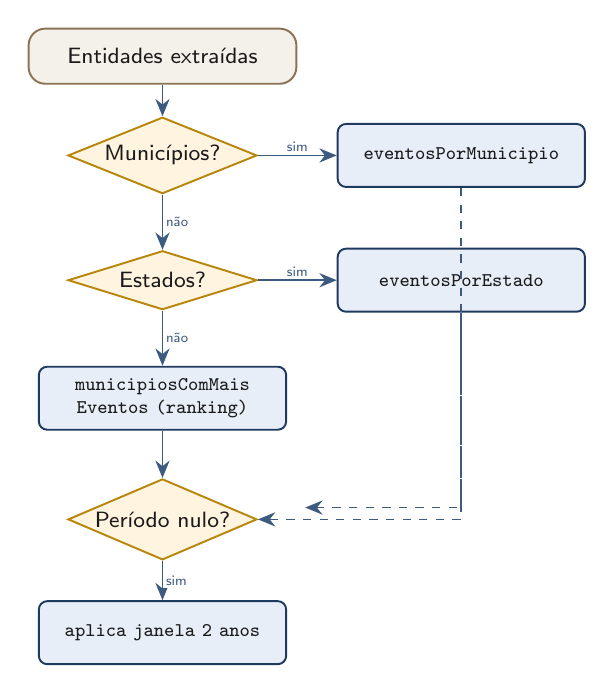
\begin{tikzpicture}[
  font=\sffamily\footnotesize,
  every node/.style={text=textDark},
  start/.style={
    rectangle, rounded corners=6pt,
    draw=softStroke, line width=0.7pt, fill=soft,
    minimum width=34mm, minimum height=7mm,
    align=center
  },
  decision/.style={
    diamond, aspect=2.2,
    draw=decisionStroke, line width=0.7pt, fill=decision,
    minimum width=24mm, inner sep=0.5pt, align=center
  },
  action/.style={
    rectangle, rounded corners=3pt,
    draw=nodeStroke, line width=0.7pt, fill=nodeFill,
    text width=30mm, minimum height=8mm, align=center,
    font=\sffamily\scriptsize\ttfamily, inner sep=2pt
  },
  flow/.style={
    -{Stealth[length=2.2mm, width=1.8mm]},
    draw=accent, line width=0.6pt
  },
  edgelabel/.style={
    font=\sffamily\tiny, text=accent,
    fill=white, inner sep=1pt
  }
]
  \node[start] (start) {Entidades extraídas};
  \node[decision, below=4mm of start] (d1) {Municípios?};
  \node[action, right=10mm of d1] (a1) {eventosPorMunicipio};
  \node[decision, below=7mm of d1] (d2) {Estados?};
  \node[action, right=10mm of d2] (a2) {eventosPorEstado};
  \node[action, below=7mm of d2] (a3) {municipiosComMais\\Eventos (ranking)};
  \node[decision, below=6mm of a3] (d3) {Período nulo?};
  \node[action, below=5mm of d3] (a4) {aplica janela 2 anos};

  \draw[flow] (start) -- (d1);
  \draw[flow] (d1.east) -- (a1.west) node[edgelabel, midway, above] {sim};
  \draw[flow] (d1.south) -- (d2.north) node[edgelabel, midway, right] {não};
  \draw[flow] (d2.east) -- (a2.west) node[edgelabel, midway, above] {sim};
  \draw[flow] (d2.south) -- (a3.north) node[edgelabel, midway, right] {não};
  \draw[flow] (a3.south) -- (d3.north);
  \draw[flow, dashed] (a1.south) |- ($(d3.east) + (8mm,0)$) -- (d3.east);
  \draw[flow, dashed] (a2.south) |- ($(d3.east) + (6mm,1.5mm)$);
  \draw[flow] (d3.south) -- (a4.north) node[edgelabel, midway, right] {sim};
\end{tikzpicture}
}
\caption{Lógica de roteamento da recuperação do subgrafo.}
\label{fig:roteamento}
\end{figure}
